\documentclass{standalone}
\usepackage{tikz}
\usetikzlibrary{patterns, positioning}
\usepackage[sfdefault]{ClearSans} %% option 'sfdefault' activates Clear Sans as the default text font
\usepackage[T1]{fontenc}

\begin{document}
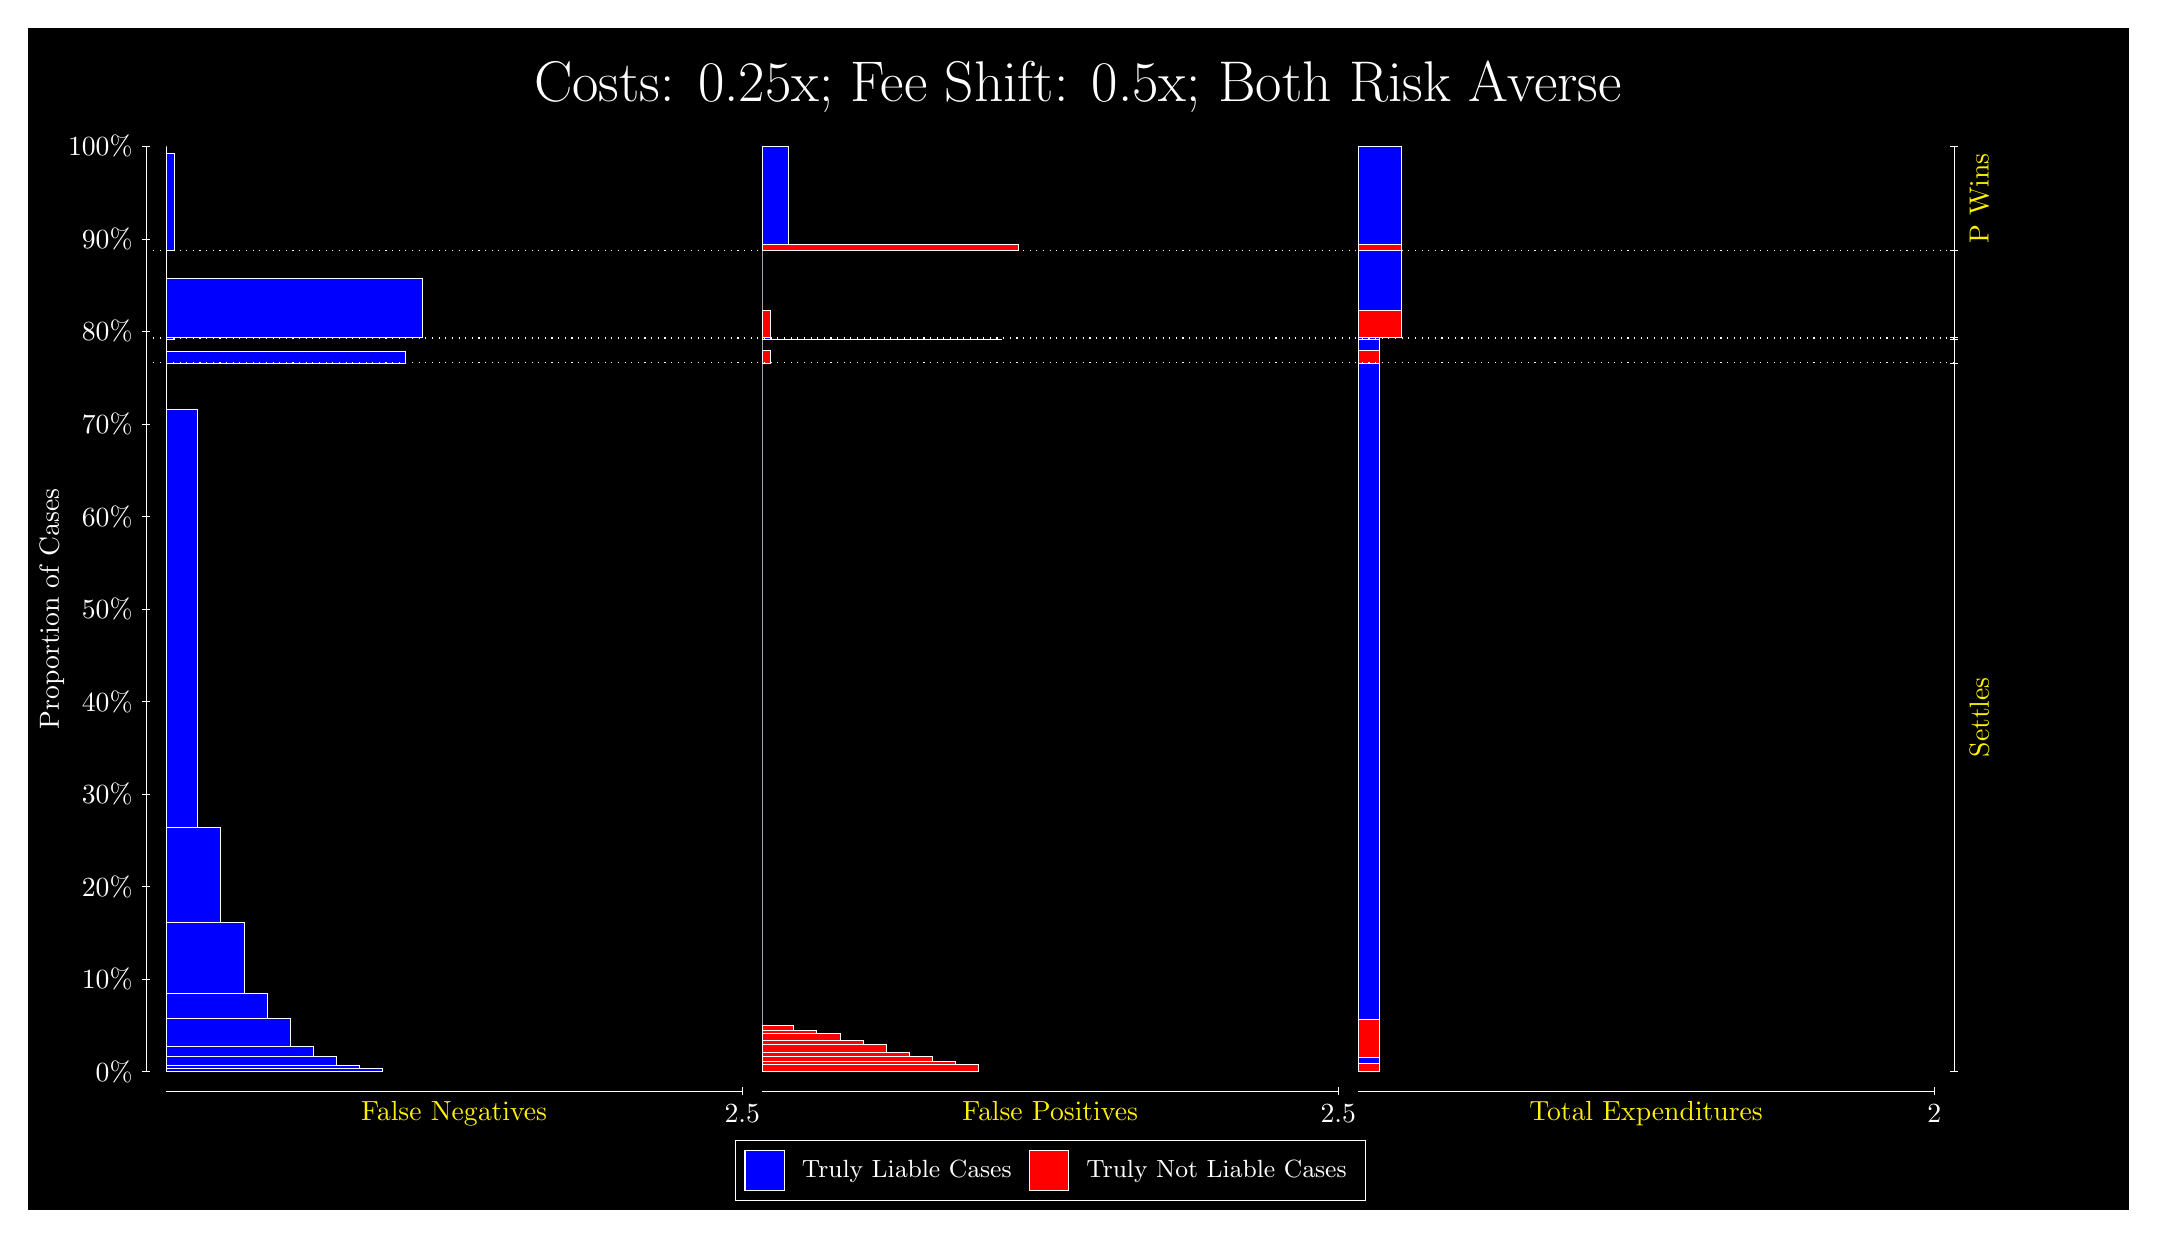
\begin{tikzpicture}
\draw[fill=black] (0,0) rectangle (26.667,15);
\draw[text=white] (0,13.5) rectangle (26.667,15) node[midway] {\huge Costs: 0.25x; Fee Shift: 0.5x; Both Risk Averse};
\draw[white, very thin] (1.5,1.75) -- (1.5,13.5);
\node[rotate=90, text=white, anchor=center] at (0.3, 7.625) {Proportion of Cases};
\draw[white, very thin] (1.45,1.75) -- (1.55,1.75);
\node[text=white, anchor=east] at (1.45, 1.75) {0\%};
\draw[white, very thin] (1.45,2.925) -- (1.55,2.925);
\node[text=white, anchor=east] at (1.45, 2.925) {10\%};
\draw[white, very thin] (1.45,4.1) -- (1.55,4.1);
\node[text=white, anchor=east] at (1.45, 4.1) {20\%};
\draw[white, very thin] (1.45,5.275) -- (1.55,5.275);
\node[text=white, anchor=east] at (1.45, 5.275) {30\%};
\draw[white, very thin] (1.45,6.45) -- (1.55,6.45);
\node[text=white, anchor=east] at (1.45, 6.45) {40\%};
\draw[white, very thin] (1.45,7.625) -- (1.55,7.625);
\node[text=white, anchor=east] at (1.45, 7.625) {50\%};
\draw[white, very thin] (1.45,8.8) -- (1.55,8.8);
\node[text=white, anchor=east] at (1.45, 8.8) {60\%};
\draw[white, very thin] (1.45,9.975) -- (1.55,9.975);
\node[text=white, anchor=east] at (1.45, 9.975) {70\%};
\draw[white, very thin] (1.45,11.15) -- (1.55,11.15);
\node[text=white, anchor=east] at (1.45, 11.15) {80\%};
\draw[white, very thin] (1.45,12.325) -- (1.55,12.325);
\node[text=white, anchor=east] at (1.45, 12.325) {90\%};
\draw[white, very thin] (1.45,13.5) -- (1.55,13.5);
\node[text=white, anchor=east] at (1.45, 13.5) {100\%};

\draw[white, very thin] (24.457,1.75) -- (24.457,13.5);
\draw[white, very thin] (24.407,1.75) -- (24.507,1.75);
\node[anchor=west] at (24.407, 1.75) {};
\draw[white, very thin] (24.407,10.75) -- (24.507,10.75);
\node[anchor=west] at (24.407, 10.75) {};
\draw[white, very thin] (24.407,11.054) -- (24.507,11.054);
\node[anchor=west] at (24.407, 11.054) {};
\draw[white, very thin] (24.407,11.07) -- (24.507,11.07);
\node[anchor=west] at (24.407, 11.07) {};
\draw[white, very thin] (24.407,12.177) -- (24.507,12.177);
\node[anchor=west] at (24.407, 12.177) {};
\draw[white, very thin] (24.407,13.5) -- (24.507,13.5);
\node[anchor=west] at (24.407, 13.5) {};

\draw[white, very thin, fill=blue] (1.75,1.75) rectangle (4.4946,1.7958);
\draw[white, very thin, fill=blue] (1.75,1.7958) rectangle (4.2018,1.8265);
\draw[white, very thin, fill=blue] (1.75,1.8265) rectangle (3.9091,1.9384);
\draw[white, very thin, fill=blue] (1.75,1.9384) rectangle (3.6163,2.065);
\draw[white, very thin, fill=blue] (1.75,2.065) rectangle (3.3236,2.4243);
\draw[white, very thin, fill=blue] (1.75,2.4243) rectangle (3.0308,2.7435);
\draw[white, very thin, fill=blue] (1.75,2.7435) rectangle (2.738,3.6438);
\draw[white, very thin, fill=blue] (1.75,3.6438) rectangle (2.4453,4.8458);
\draw[white, very thin, fill=blue] (1.75,4.8458) rectangle (2.1525,10.165);
\draw[white, very thin, fill=red] (1.75,10.165) rectangle (1.75,10.75);
\draw[white, very thin, fill=blue] (1.75,10.75) rectangle (4.7873,10.899);
\draw[white, very thin, fill=red] (1.75,10.899) rectangle (1.75,11.054);
\draw[white, very thin, fill=blue] (1.75,11.054) rectangle (1.8598,11.069);
\draw[white, very thin, fill=red] (1.75,11.069) rectangle (1.75,11.07);
\draw[white, very thin, fill=blue] (1.75,11.07) rectangle (5.0069,11.825);
\draw[white, very thin, fill=red] (1.75,11.825) rectangle (1.75,12.177);
\draw[white, very thin, fill=blue] (1.75,12.177) rectangle (1.8598,13.417);
\draw[white, very thin, fill=red] (1.75,13.417) rectangle (1.75,13.5);
\draw[white, very thin, fill=red] (9.3189,1.75) rectangle (12.063,1.8381);
\draw[white, very thin, fill=red] (9.3189,1.8381) rectangle (11.771,1.8798);
\draw[white, very thin, fill=red] (9.3189,1.8798) rectangle (11.478,1.9483);
\draw[white, very thin, fill=red] (9.3189,1.9483) rectangle (11.185,1.9974);
\draw[white, very thin, fill=red] (9.3189,1.9974) rectangle (10.892,2.0975);
\draw[white, very thin, fill=red] (9.3189,2.0975) rectangle (10.6,2.1456);
\draw[white, very thin, fill=red] (9.3189,2.1456) rectangle (10.6,2.1517);
\draw[white, very thin, fill=red] (9.3189,2.1517) rectangle (10.307,2.2332);
\draw[white, very thin, fill=red] (9.3189,2.2332) rectangle (10.014,2.2681);
\draw[white, very thin, fill=red] (9.3189,2.2681) rectangle (9.7214,2.3349);
\draw[white, very thin, fill=blue] (9.3189,2.3349) rectangle (9.3189,10.75);
\draw[white, very thin, fill=red] (9.3189,10.75) rectangle (9.4287,10.905);
\draw[white, very thin, fill=blue] (9.3189,10.905) rectangle (9.3189,11.054);
\draw[white, very thin, fill=red] (9.3189,11.054) rectangle (12.356,11.055);
\draw[white, very thin, fill=blue] (9.3189,11.055) rectangle (9.4287,11.07);
\draw[white, very thin, fill=red] (9.3189,11.07) rectangle (9.4287,11.421);
\draw[white, very thin, fill=blue] (9.3189,11.421) rectangle (9.3189,12.177);
\draw[white, very thin, fill=red] (9.3189,12.177) rectangle (12.576,12.259);
\draw[white, very thin, fill=blue] (9.3189,12.259) rectangle (9.6482,13.5);
\draw[white, very thin, fill=red] (16.888,1.75) rectangle (17.162,1.8516);
\draw[white, very thin, fill=blue] (16.888,1.8516) rectangle (17.162,1.9282);
\draw[white, very thin, fill=red] (16.888,1.9282) rectangle (17.162,2.4114);
\draw[white, very thin, fill=blue] (16.888,2.4114) rectangle (17.162,10.75);
\draw[white, very thin, fill=red] (16.888,10.75) rectangle (17.162,10.905);
\draw[white, very thin, fill=blue] (16.888,10.905) rectangle (17.162,11.054);
\draw[white, very thin, fill=red] (16.888,11.054) rectangle (17.162,11.055);
\draw[white, very thin, fill=blue] (16.888,11.055) rectangle (17.162,11.07);
\draw[white, very thin, fill=red] (16.888,11.07) rectangle (17.437,11.421);
\draw[white, very thin, fill=blue] (16.888,11.421) rectangle (17.437,12.177);
\draw[white, very thin, fill=red] (16.888,12.177) rectangle (17.437,12.259);
\draw[white, very thin, fill=blue] (16.888,12.259) rectangle (17.437,13.5);
\draw[white, dotted] (1.5,10.75) -- (24.457,10.75);
\draw[white, dotted] (1.5,11.054) -- (24.457,11.054);
\draw[white, dotted] (1.5,11.07) -- (24.457,11.07);
\draw[white, dotted] (1.5,12.177) -- (24.457,12.177);
\draw[white, very thin] (1.75,1.5) -- (9.0689,1.5);
\node[text=yellow, anchor=north] at (5.4094, 1.5) {False Negatives};
\draw[white, very thin] (9.0689,1.45) -- (9.0689,1.55);
\node[text=white, anchor=north] at (9.0689, 1.45) {2.5};

\draw[white, very thin] (9.3189,1.5) -- (16.638,1.5);
\node[text=yellow, anchor=north] at (12.978, 1.5) {False Positives};
\draw[white, very thin] (16.638,1.45) -- (16.638,1.55);
\node[text=white, anchor=north] at (16.638, 1.45) {2.5};

\draw[white, very thin] (16.888,1.5) -- (24.207,1.5);
\node[text=yellow, anchor=north] at (20.547, 1.5) {Total Expenditures};
\draw[white, very thin] (24.207,1.45) -- (24.207,1.55);
\node[text=white, anchor=north] at (24.207, 1.45) {2};

\node[text=yellow, centered, rotate=90] at (24.777, 6.2499) {Settles};



\node[text=yellow, centered, rotate=90] at (24.777, 12.838) {P Wins};

\draw (12.978300999999998,1.5) node[draw=none] (baseCoordinate) {};
\begin{scope}[align=center]
        \matrix[scale=0.5, draw=white, below=0.5cm of baseCoordinate, nodes={draw}, column sep=0.1cm]{
            \node[rectangle, draw, minimum width=0.5cm, minimum height=0.5cm, fill=blue] {}; &
            \node[draw=none, font=\small, text=white] (B) {Truly Liable Cases}; &
            \node[rectangle, draw, minimum width=0.5cm, minimum height=0.5cm, fill=red] {}; &
            \node[draw=none, font=\small, text=white] (B) {Truly Not Liable Cases}; \\
            };
\end{scope}

\end{tikzpicture}
\end{document}